\documentclass[border=10pt]{standalone}
\usepackage{tikz}
\usetikzlibrary{arrows.meta,calc}

\begin{document}
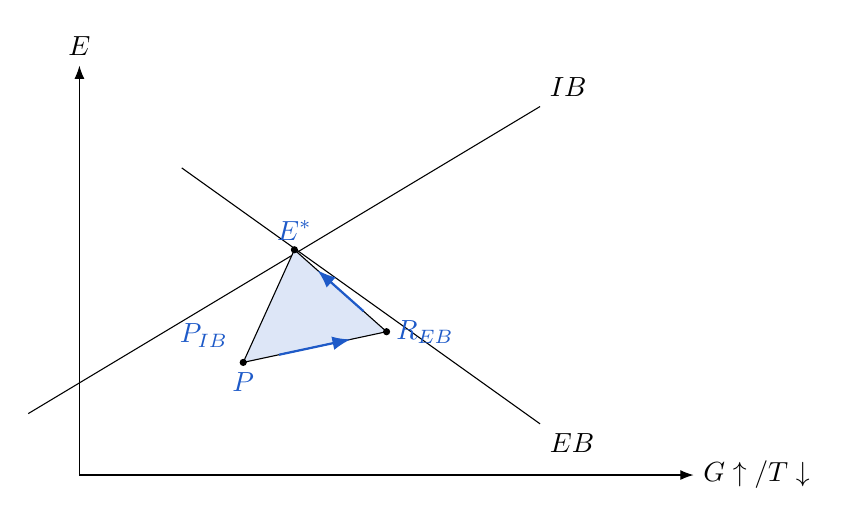
\begin{tikzpicture}[>=Latex,scale=1.3]

% Colors
\definecolor{myblue}{RGB}{30,90,200}

% Axes
\draw[->] (0,0) -- (0,4) node[above] {$E$};
\draw[->] (0,0) -- (6,0) node[right] {$G\uparrow/T\downarrow$};

% Helper coordinates for triangle vertices
\coordinate (P)  at (1.6,1.1);
\coordinate (E)  at (2.1,2.2);
\coordinate (REB) at (3.0,1.4);

% Diagonal lines IB and EB
% IB: upward sloping through E
\draw (-0.5,0.6) -- (4.5,3.6) node[above right] {$IB$};
% EB: downward sloping through R_EB
\draw (1.0,3.0) -- (4.5,0.5) node[below right] {$EB$};

% Triangle (filled lightly in blue)
\fill[myblue!15] (P) -- (E) -- (REB) -- cycle;
\draw (P) -- (E) -- (REB) -- cycle;

% Blue arrows along triangle edges
\draw[->,myblue,thick] ($(P)!0.25!(REB)$) -- ($(P)!0.75!(REB)$);
\draw[->,myblue,thick] ($(REB)!0.25!(E)$) -- ($(REB)!0.75!(E)$);

% Point markers
\fill (P) circle (1pt);
\fill (E) circle (1pt);
\fill (REB) circle (1pt);

% Blue labels for points
\node[below, myblue] at (P) {$P$};
\node[above left=2pt, myblue] at (P) {$P_{IB}$};
\node[above, myblue] at (E) {$E^{*}$};
\node[right, myblue] at (REB) {$R_{EB}$};

\end{tikzpicture}
\end{document}